\documentclass[lettersize,journal]{IEEEtran}
\usepackage{amsmath,amsfonts}
\usepackage{array}
\usepackage{booktabs}
\usepackage{multirow}
\usepackage{xcolor}
\usepackage{graphicx}
\usepackage{url}
\usepackage{cite}
\usepackage{tikz}
\usetikzlibrary{arrows.meta,positioning,shapes.misc,calc,fit}
\usepackage{balance}
% AUTO-GENERATED by evaluation/make_results_tex.py — do not edit
\newcommand{\NA}{\textcolor{red}{n/a}}
\newcommand{\MEmulBoneortfpthreetwocpuMedian}{0.547}
\newcommand{\MEmulBoneortfpthreetwocpuPninenine}{0.620}
\newcommand{\MEmulBoneortfpthreetwocpuCV}{\NA}
\newcommand{\MEmulBoneortfpthreetwocpuPower}{6,510}
\newcommand{\MEmulBoneortfpthreetwocpuSamples}{28}
\newcommand{\MEmulBoneortfpthreetwocpuEnergy}{3.63}
\newcommand{\MEmulBoneortfpthreetwocpuLinkOut}{\NA}
\newcommand{\MEmulBoneortfpthreetwocpuLinkIn}{\NA}
\newcommand{\MEmulBoneortfpthreetwocpuMsgs}{\NA}
\newcommand{\MEmulBoneortfpthreetwocpuFaults}{\NA}
\newcommand{\MEmulBoneortfpthreetwocpuPrepare}{0}
\newcommand{\MEmulBoneortfpthreetwocpuBitExact}{\NA}
\newcommand{\MEmulBoneortfpthreetwocpuNormErr}{\NA}
\newcommand{\MEmulBoneortfpthreetwocpuStatus}{ok}
\newcommand{\MEmulBtwoortinteightcpuMedian}{0.270}
\newcommand{\MEmulBtwoortinteightcpuPninenine}{0.692}
\newcommand{\MEmulBtwoortinteightcpuCV}{\NA}
\newcommand{\MEmulBtwoortinteightcpuPower}{6,142}
\newcommand{\MEmulBtwoortinteightcpuSamples}{63}
\newcommand{\MEmulBtwoortinteightcpuEnergy}{1.83}
\newcommand{\MEmulBtwoortinteightcpuLinkOut}{\NA}
\newcommand{\MEmulBtwoortinteightcpuLinkIn}{\NA}
\newcommand{\MEmulBtwoortinteightcpuMsgs}{\NA}
\newcommand{\MEmulBtwoortinteightcpuFaults}{\NA}
\newcommand{\MEmulBtwoortinteightcpuPrepare}{0}
\newcommand{\MEmulBtwoortinteightcpuBitExact}{\NA}
\newcommand{\MEmulBtwoortinteightcpuNormErr}{\NA}
\newcommand{\MEmulBtwoortinteightcpuStatus}{ok}
\newcommand{\MEmulBthreetrtfponesixgpuMedian}{0.448}
\newcommand{\MEmulBthreetrtfponesixgpuPninenine}{1.57}
\newcommand{\MEmulBthreetrtfponesixgpuCV}{58}
\newcommand{\MEmulBthreetrtfponesixgpuPower}{6,036}
\newcommand{\MEmulBthreetrtfponesixgpuSamples}{30}
\newcommand{\MEmulBthreetrtfponesixgpuEnergy}{3.01}
\newcommand{\MEmulBthreetrtfponesixgpuLinkOut}{\NA}
\newcommand{\MEmulBthreetrtfponesixgpuLinkIn}{\NA}
\newcommand{\MEmulBthreetrtfponesixgpuMsgs}{\NA}
\newcommand{\MEmulBthreetrtfponesixgpuFaults}{\NA}
\newcommand{\MEmulBthreetrtfponesixgpuPrepare}{0}
\newcommand{\MEmulBthreetrtfponesixgpuBitExact}{\NA}
\newcommand{\MEmulBthreetrtfponesixgpuNormErr}{\NA}
\newcommand{\MEmulBthreetrtfponesixgpuStatus}{ok}
\newcommand{\MEmulBfourtrtinteightgpuMedian}{0.403}
\newcommand{\MEmulBfourtrtinteightgpuPninenine}{4.65}
\newcommand{\MEmulBfourtrtinteightgpuCV}{147}
\newcommand{\MEmulBfourtrtinteightgpuPower}{6,359}
\newcommand{\MEmulBfourtrtinteightgpuSamples}{30}
\newcommand{\MEmulBfourtrtinteightgpuEnergy}{4.72}
\newcommand{\MEmulBfourtrtinteightgpuLinkOut}{\NA}
\newcommand{\MEmulBfourtrtinteightgpuLinkIn}{\NA}
\newcommand{\MEmulBfourtrtinteightgpuMsgs}{\NA}
\newcommand{\MEmulBfourtrtinteightgpuFaults}{\NA}
\newcommand{\MEmulBfourtrtinteightgpuPrepare}{0}
\newcommand{\MEmulBfourtrtinteightgpuBitExact}{\NA}
\newcommand{\MEmulBfourtrtinteightgpuNormErr}{\NA}
\newcommand{\MEmulBfourtrtinteightgpuStatus}{ok}
\newcommand{\MEmulSIhostMedian}{1.64}
\newcommand{\MEmulSIhostPninenine}{1.65}
\newcommand{\MEmulSIhostCV}{0}
\newcommand{\MEmulSIhostPower}{6,003}
\newcommand{\MEmulSIhostSamples}{26}
\newcommand{\MEmulSIhostEnergy}{9.85}
\newcommand{\MEmulSIhostLinkOut}{0}
\newcommand{\MEmulSIhostLinkIn}{0}
\newcommand{\MEmulSIhostMsgs}{0}
\newcommand{\MEmulSIhostFaults}{0}
\newcommand{\MEmulSIhostPrepare}{0}
\newcommand{\MEmulSIhostBitExact}{3/3}
\newcommand{\MEmulSIhostNormErr}{0.061}
\newcommand{\MEmulSIhostStatus}{ok}
\newcommand{\EEmulSInmcMedian}{551}
\newcommand{\EEmulSInmcPninenine}{552}
\newcommand{\EEmulSInmcCV}{0}
\newcommand{\EEmulSInmcPower}{5,387}
\newcommand{\EEmulSInmcSamples}{2988}
\newcommand{\EEmulSInmcEnergy}{2970.72}
\newcommand{\EEmulSInmcLinkOut}{1,907}
\newcommand{\EEmulSInmcLinkIn}{476}
\newcommand{\EEmulSInmcMsgs}{59}
\newcommand{\EEmulSInmcFaults}{0}
\newcommand{\EEmulSInmcPrepare}{334}
\newcommand{\EEmulSInmcBitExact}{3/3}
\newcommand{\EEmulSInmcNormErr}{0.061}
\newcommand{\EEmulSInmcStatus}{ok}
\newcommand{\EEmulSIpoolMedian}{307,666}
\newcommand{\EEmulSIpoolPninenine}{309,060}
\newcommand{\EEmulSIpoolCV}{1}
\newcommand{\EEmulSIpoolPower}{5,191}
\newcommand{\EEmulSIpoolSamples}{16663}
\newcommand{\EEmulSIpoolEnergy}{1593371.75}
\newcommand{\EEmulSIpoolLinkOut}{0}
\newcommand{\EEmulSIpoolLinkIn}{3,534,848}
\newcommand{\EEmulSIpoolMsgs}{14}
\newcommand{\EEmulSIpoolFaults}{14}
\newcommand{\EEmulSIpoolPrepare}{334}
\newcommand{\EEmulSIpoolBitExact}{3/3}
\newcommand{\EEmulSIpoolNormErr}{0.061}
\newcommand{\EEmulSIpoolStatus}{ok}
\newcommand{\EEmulSIpoolwarmMedian}{1,440}
\newcommand{\EEmulSIpoolwarmPninenine}{4,228}
\newcommand{\EEmulSIpoolwarmCV}{69}
\newcommand{\EEmulSIpoolwarmPower}{5,226}
\newcommand{\EEmulSIpoolwarmSamples}{5848}
\newcommand{\EEmulSIpoolwarmEnergy}{12469.01}
\newcommand{\EEmulSIpoolwarmLinkOut}{0}
\newcommand{\EEmulSIpoolwarmLinkIn}{27,307}
\newcommand{\EEmulSIpoolwarmMsgs}{2}
\newcommand{\EEmulSIpoolwarmFaults}{2}
\newcommand{\EEmulSIpoolwarmPrepare}{334}
\newcommand{\EEmulSIpoolwarmBitExact}{3/3}
\newcommand{\EEmulSIpoolwarmNormErr}{0.061}
\newcommand{\EEmulSIpoolwarmStatus}{ok}
\newcommand{\MUsbBoneortfpthreetwocpuMedian}{\NA}
\newcommand{\MUsbBoneortfpthreetwocpuPninenine}{\NA}
\newcommand{\MUsbBoneortfpthreetwocpuCV}{\NA}
\newcommand{\MUsbBoneortfpthreetwocpuPower}{\NA}
\newcommand{\MUsbBoneortfpthreetwocpuSamples}{\NA}
\newcommand{\MUsbBoneortfpthreetwocpuEnergy}{\NA}
\newcommand{\MUsbBoneortfpthreetwocpuLinkOut}{\NA}
\newcommand{\MUsbBoneortfpthreetwocpuLinkIn}{\NA}
\newcommand{\MUsbBoneortfpthreetwocpuMsgs}{\NA}
\newcommand{\MUsbBoneortfpthreetwocpuFaults}{\NA}
\newcommand{\MUsbBoneortfpthreetwocpuPrepare}{0}
\newcommand{\MUsbBoneortfpthreetwocpuBitExact}{\NA}
\newcommand{\MUsbBoneortfpthreetwocpuNormErr}{\NA}
\newcommand{\MUsbBoneortfpthreetwocpuStatus}{missing}
\newcommand{\MUsbBtwoortinteightcpuMedian}{\NA}
\newcommand{\MUsbBtwoortinteightcpuPninenine}{\NA}
\newcommand{\MUsbBtwoortinteightcpuCV}{\NA}
\newcommand{\MUsbBtwoortinteightcpuPower}{\NA}
\newcommand{\MUsbBtwoortinteightcpuSamples}{\NA}
\newcommand{\MUsbBtwoortinteightcpuEnergy}{\NA}
\newcommand{\MUsbBtwoortinteightcpuLinkOut}{\NA}
\newcommand{\MUsbBtwoortinteightcpuLinkIn}{\NA}
\newcommand{\MUsbBtwoortinteightcpuMsgs}{\NA}
\newcommand{\MUsbBtwoortinteightcpuFaults}{\NA}
\newcommand{\MUsbBtwoortinteightcpuPrepare}{0}
\newcommand{\MUsbBtwoortinteightcpuBitExact}{\NA}
\newcommand{\MUsbBtwoortinteightcpuNormErr}{\NA}
\newcommand{\MUsbBtwoortinteightcpuStatus}{missing}
\newcommand{\MUsbBthreetrtfponesixgpuMedian}{\NA}
\newcommand{\MUsbBthreetrtfponesixgpuPninenine}{\NA}
\newcommand{\MUsbBthreetrtfponesixgpuCV}{\NA}
\newcommand{\MUsbBthreetrtfponesixgpuPower}{\NA}
\newcommand{\MUsbBthreetrtfponesixgpuSamples}{\NA}
\newcommand{\MUsbBthreetrtfponesixgpuEnergy}{\NA}
\newcommand{\MUsbBthreetrtfponesixgpuLinkOut}{\NA}
\newcommand{\MUsbBthreetrtfponesixgpuLinkIn}{\NA}
\newcommand{\MUsbBthreetrtfponesixgpuMsgs}{\NA}
\newcommand{\MUsbBthreetrtfponesixgpuFaults}{\NA}
\newcommand{\MUsbBthreetrtfponesixgpuPrepare}{0}
\newcommand{\MUsbBthreetrtfponesixgpuBitExact}{\NA}
\newcommand{\MUsbBthreetrtfponesixgpuNormErr}{\NA}
\newcommand{\MUsbBthreetrtfponesixgpuStatus}{missing}
\newcommand{\MUsbBfourtrtinteightgpuMedian}{\NA}
\newcommand{\MUsbBfourtrtinteightgpuPninenine}{\NA}
\newcommand{\MUsbBfourtrtinteightgpuCV}{\NA}
\newcommand{\MUsbBfourtrtinteightgpuPower}{\NA}
\newcommand{\MUsbBfourtrtinteightgpuSamples}{\NA}
\newcommand{\MUsbBfourtrtinteightgpuEnergy}{\NA}
\newcommand{\MUsbBfourtrtinteightgpuLinkOut}{\NA}
\newcommand{\MUsbBfourtrtinteightgpuLinkIn}{\NA}
\newcommand{\MUsbBfourtrtinteightgpuMsgs}{\NA}
\newcommand{\MUsbBfourtrtinteightgpuFaults}{\NA}
\newcommand{\MUsbBfourtrtinteightgpuPrepare}{0}
\newcommand{\MUsbBfourtrtinteightgpuBitExact}{\NA}
\newcommand{\MUsbBfourtrtinteightgpuNormErr}{\NA}
\newcommand{\MUsbBfourtrtinteightgpuStatus}{missing}
\newcommand{\MUsbSIhostMedian}{\NA}
\newcommand{\MUsbSIhostPninenine}{\NA}
\newcommand{\MUsbSIhostCV}{\NA}
\newcommand{\MUsbSIhostPower}{\NA}
\newcommand{\MUsbSIhostSamples}{\NA}
\newcommand{\MUsbSIhostEnergy}{\NA}
\newcommand{\MUsbSIhostLinkOut}{\NA}
\newcommand{\MUsbSIhostLinkIn}{\NA}
\newcommand{\MUsbSIhostMsgs}{\NA}
\newcommand{\MUsbSIhostFaults}{\NA}
\newcommand{\MUsbSIhostPrepare}{0}
\newcommand{\MUsbSIhostBitExact}{\NA}
\newcommand{\MUsbSIhostNormErr}{\NA}
\newcommand{\MUsbSIhostStatus}{missing}
\newcommand{\MUsbSInmcMedian}{\NA}
\newcommand{\MUsbSInmcPninenine}{\NA}
\newcommand{\MUsbSInmcCV}{\NA}
\newcommand{\MUsbSInmcPower}{\NA}
\newcommand{\MUsbSInmcSamples}{\NA}
\newcommand{\MUsbSInmcEnergy}{\NA}
\newcommand{\MUsbSInmcLinkOut}{\NA}
\newcommand{\MUsbSInmcLinkIn}{\NA}
\newcommand{\MUsbSInmcMsgs}{\NA}
\newcommand{\MUsbSInmcFaults}{\NA}
\newcommand{\MUsbSInmcPrepare}{0}
\newcommand{\MUsbSInmcBitExact}{\NA}
\newcommand{\MUsbSInmcNormErr}{\NA}
\newcommand{\MUsbSInmcStatus}{missing}
\newcommand{\MUsbSIpoolMedian}{\NA}
\newcommand{\MUsbSIpoolPninenine}{\NA}
\newcommand{\MUsbSIpoolCV}{\NA}
\newcommand{\MUsbSIpoolPower}{\NA}
\newcommand{\MUsbSIpoolSamples}{\NA}
\newcommand{\MUsbSIpoolEnergy}{\NA}
\newcommand{\MUsbSIpoolLinkOut}{\NA}
\newcommand{\MUsbSIpoolLinkIn}{\NA}
\newcommand{\MUsbSIpoolMsgs}{\NA}
\newcommand{\MUsbSIpoolFaults}{\NA}
\newcommand{\MUsbSIpoolPrepare}{0}
\newcommand{\MUsbSIpoolBitExact}{\NA}
\newcommand{\MUsbSIpoolNormErr}{\NA}
\newcommand{\MUsbSIpoolStatus}{missing}
\newcommand{\MUsbSIpoolwarmMedian}{\NA}
\newcommand{\MUsbSIpoolwarmPninenine}{\NA}
\newcommand{\MUsbSIpoolwarmCV}{\NA}
\newcommand{\MUsbSIpoolwarmPower}{\NA}
\newcommand{\MUsbSIpoolwarmSamples}{\NA}
\newcommand{\MUsbSIpoolwarmEnergy}{\NA}
\newcommand{\MUsbSIpoolwarmLinkOut}{\NA}
\newcommand{\MUsbSIpoolwarmLinkIn}{\NA}
\newcommand{\MUsbSIpoolwarmMsgs}{\NA}
\newcommand{\MUsbSIpoolwarmFaults}{\NA}
\newcommand{\MUsbSIpoolwarmPrepare}{0}
\newcommand{\MUsbSIpoolwarmBitExact}{\NA}
\newcommand{\MUsbSIpoolwarmNormErr}{\NA}
\newcommand{\MUsbSIpoolwarmStatus}{missing}
\newcommand{\Esixuartoneonefivetwozerozeronmc}{551}
\newcommand{\EsixuartoneonefivetwozerozeronmcFaults}{0}
\newcommand{\Esixuartoneonefivetwozerozeropoolpfone}{196,769}
\newcommand{\EsixuartoneonefivetwozerozeropoolpfoneFaults}{542}
\newcommand{\Esixuartoneonefivetwozerozeropoolpfsixfour}{310,512}
\newcommand{\EsixuartoneonefivetwozerozeropoolpfsixfourFaults}{14}
\newcommand{\Esixuartoneonefivetwozerozeropoolpffiveonetwo}{326,422}
\newcommand{\EsixuartoneonefivetwozerozeropoolpffiveonetwoFaults}{2}
\newcommand{\Esixuartoneonefivetwozerozeropoolwarm}{7,500}
\newcommand{\EsixuartoneonefivetwozerozeropoolwarmFaults}{4}
\newcommand{\Esixuartninetwoonesixzerozeronmc}{134}
\newcommand{\EsixuartninetwoonesixzerozeronmcFaults}{0}
\newcommand{\Esixuartninetwoonesixzerozeropoolpfone}{24,935}
\newcommand{\EsixuartninetwoonesixzerozeropoolpfoneFaults}{542}
\newcommand{\Esixuartninetwoonesixzerozeropoolpfsixfour}{38,829}
\newcommand{\EsixuartninetwoonesixzerozeropoolpfsixfourFaults}{14}
\newcommand{\Esixuartninetwoonesixzerozeropoolpffiveonetwo}{40,810}
\newcommand{\EsixuartninetwoonesixzerozeropoolpffiveonetwoFaults}{2}
\newcommand{\Esixuartninetwoonesixzerozeropoolwarm}{943}
\newcommand{\EsixuartninetwoonesixzerozeropoolwarmFaults}{4}
\newcommand{\Esixusbtwobulknmc}{77.6}
\newcommand{\EsixusbtwobulknmcFaults}{0}
\newcommand{\Esixusbtwobulkpoolpfone}{437}
\newcommand{\EsixusbtwobulkpoolpfoneFaults}{542}
\newcommand{\Esixusbtwobulkpoolpfsixfour}{135}
\newcommand{\EsixusbtwobulkpoolpfsixfourFaults}{14}
\newcommand{\Esixusbtwobulkpoolpffiveonetwo}{133}
\newcommand{\EsixusbtwobulkpoolpffiveonetwoFaults}{2}
\newcommand{\Esixusbtwobulkpoolwarm}{4.90}
\newcommand{\EsixusbtwobulkpoolwarmFaults}{2}
\newcommand{\Esixusbthreenmc}{54.1}
\newcommand{\EsixusbthreenmcFaults}{0}
\newcommand{\Esixusbthreepoolpfone}{151}
\newcommand{\EsixusbthreepoolpfoneFaults}{542}
\newcommand{\Esixusbthreepoolpfsixfour}{21.8}
\newcommand{\EsixusbthreepoolpfsixfourFaults}{14}
\newcommand{\Esixusbthreepoolpffiveonetwo}{17.5}
\newcommand{\EsixusbthreepoolpffiveonetwoFaults}{2}
\newcommand{\Esixusbthreepoolwarm}{3.48}
\newcommand{\EsixusbthreepoolwarmFaults}{2}
\newcommand{\Esixpciethreexonenmc}{48.9}
\newcommand{\EsixpciethreexonenmcFaults}{0}
\newcommand{\Esixpciethreexonepoolpfone}{95.5}
\newcommand{\EsixpciethreexonepoolpfoneFaults}{542}
\newcommand{\Esixpciethreexonepoolpfsixfour}{10.9}
\newcommand{\EsixpciethreexonepoolpfsixfourFaults}{14}
\newcommand{\Esixpciethreexonepoolpffiveonetwo}{11.2}
\newcommand{\EsixpciethreexonepoolpffiveonetwoFaults}{2}
\newcommand{\Esixpciethreexonepoolwarm}{2.88}
\newcommand{\EsixpciethreexonepoolwarmFaults}{2}
\newcommand{\Esixpciefourxfournmc}{48.3}
\newcommand{\EsixpciefourxfournmcFaults}{0}
\newcommand{\Esixpciefourxfourpoolpfone}{89.7}
\newcommand{\EsixpciefourxfourpoolpfoneFaults}{542}
\newcommand{\Esixpciefourxfourpoolpfsixfour}{8.68}
\newcommand{\EsixpciefourxfourpoolpfsixfourFaults}{14}
\newcommand{\Esixpciefourxfourpoolpffiveonetwo}{6.26}
\newcommand{\EsixpciefourxfourpoolpffiveonetwoFaults}{2}
\newcommand{\Esixpciefourxfourpoolwarm}{2.61}
\newcommand{\EsixpciefourxfourpoolwarmFaults}{2}
\newcommand{\EsevenhostMedian}{162}
\newcommand{\EsevenhostStream}{0.000}
\newcommand{\EsevenhostBitExact}{4/4}
\newcommand{\EsevenhostNormErr}{0.082}
\newcommand{\EsevennmcnolinkMedian}{124}
\newcommand{\EsevennmcnolinkStream}{58.4}
\newcommand{\EsevennmcnolinkBitExact}{4/4}
\newcommand{\EsevennmcnolinkNormErr}{0.082}
\newcommand{\EsevennmcusbtwoMedian}{35,927}
\newcommand{\EsevennmcusbtwoStream}{32,631}
\newcommand{\EsevennmcusbtwoBitExact}{2/2}
\newcommand{\EsevennmcusbtwoNormErr}{0.101}
\newcommand{\EsevennmcusbthreeMedian}{13,188}
\newcommand{\EsevennmcusbthreeStream}{9,905}
\newcommand{\EsevennmcusbthreeBitExact}{2/2}
\newcommand{\EsevennmcusbthreeNormErr}{0.101}
\newcommand{\MTrtfponesixMedian}{0.396}
\newcommand{\MTrtfponesixPower}{6,568}
\newcommand{\MTrtinteightMedian}{0.411}
\newcommand{\MTrtinteightPower}{6,559}
\newcommand{\CDlrmLatency}{1,081}
\newcommand{\CDlrmWeightsMiB}{14.4}
\newcommand{\CDlrmNumGpu}{2}
\newcommand{\CDlrmNumPool}{1}
\newcommand{\CDlrmNumFpga}{33}
\newcommand{\CDlrmTransfers}{3}
\newcommand{\CDlrmBdgpucompute}{0.0}
\newcommand{\CDlrmBdfpgacompute}{37.8}
\newcommand{\CDlrmBdpoolfault}{8.3}
\newcommand{\CDlrmBdweightstream}{0.0}
\newcommand{\CDlrmBddispatch}{358.1}
\newcommand{\CDlrmBdactivationxfer}{676.7}
\newcommand{\CDlrmLinkBw}{11,520}
\newcommand{\CDlrmRtt}{8.0}
\newcommand{\CDlrmFpgaGops}{0.111}
\newcommand{\CMlpEightLatency}{61,662,272}
\newcommand{\CMlpEightWeightsMiB}{668.0}
\newcommand{\CMlpEightNumGpu}{1}
\newcommand{\CMlpEightNumPool}{0}
\newcommand{\CMlpEightNumFpga}{23}
\newcommand{\CMlpEightTransfers}{1}
\newcommand{\CMlpEightBdgpucompute}{0.0}
\newcommand{\CMlpEightBdfpgacompute}{3,155.2}
\newcommand{\CMlpEightBdpoolfault}{0.0}
\newcommand{\CMlpEightBdweightstream}{61,658,925.0}
\newcommand{\CMlpEightBddispatch}{180.9}
\newcommand{\CMlpEightBdactivationxfer}{10.6}
\newcommand{\CMlpEightLinkBw}{11,520}
\newcommand{\CMlpEightRtt}{5.0}
\newcommand{\CMlpEightFpgaGops}{0.111}
\newcommand{\PDlrmImageMiB}{3.6}
\newcommand{\PDlrmLayoutMiB}{3.6}
\newcommand{\PDlrmSlotMiB}{0.0}
\newcommand{\PDlrmTotalWeightMiB}{3.6}
\newcommand{\PDlrmNormErr}{0.127}
\newcommand{\PDlrmLayers}{30}
\newcommand{\PMlpEightImageMiB}{167.6}
\newcommand{\PMlpEightLayoutMiB}{48.0}
\newcommand{\PMlpEightSlotMiB}{23.9}
\newcommand{\PMlpEightTotalWeightMiB}{167.6}
\newcommand{\PMlpEightNormErr}{0.113}
\newcommand{\PMlpEightLayers}{8}
\newcommand{\MCapfourpfiveeightLat}{273}
\newcommand{\MCapfourpfiveeightRss}{6,046}
\newcommand{\MCapfourpfiveeightStatus}{ok}
\newcommand{\MCapsixpzerozeroLat}{1,982}
\newcommand{\MCapsixpzerozeroRss}{6,157}
\newcommand{\MCapsixpzerozeroStatus}{ok_thrashing}
\newcommand{\MCapninepthreenineLat}{\NA}
\newcommand{\MCapninepthreenineRss}{7,373}
\newcommand{\MCapninepthreenineStatus}{oom_killed}

\hyphenation{Split-Infer Edge-Coh cxl-win}
\newcommand{\cxlwin}{\textsc{cxlwin}}
\newcommand{\M}{\textsuperscript{M}}
\newcommand{\E}{\textsuperscript{E}}
\newcommand{\Cm}{\textsuperscript{C}}

\begin{document}

\title{SplitInfer: Moving Memory to Compute, or Compute to Memory?\\
A Measured Crossover for Edge Inference Beyond SoC Memory}

\author{Hemraj~Lamkuche
\thanks{Manuscript submitted to IEEE Transactions on Computers, 2026.}
\thanks{Source code, RTL, emulator, and every script that produced a number in this paper: \texttt{github.com/crypto0010/CXL}.}}

\markboth{IEEE Transactions on Computers}{Lamkuche: SplitInfer}
\maketitle

\begin{abstract}
When a model's weights exceed an edge SoC's unified memory, the system has two choices: move the memory to the compute, or move the compute to the memory. Which is cheaper is not a property of the accelerator; it is a property of the interconnect. This paper builds \emph{both} paths over one substrate and measures where they cross. The substrate is a Jetson Orin Nano attached to a commodity FPGA memory node (Nexys~4 DDR, 128~MB DDR2) by a deliberately slow UART link. \cxlwin{} maps the FPGA's DDR2 into the host address space so that ordinary loads and stores reach device memory through page faults, with an explicit host-bias/device-bias ownership model in the manner of CXL.mem Type~2 devices---stated as a page-granular software analogy, not as equivalence. Near-memory engines on the FPGA execute INT8 embedding gathers, an 8$\times$8 MAC array, and a fused requantisation epilogue. An INT8 lowering produces a single program that executes in three modes---host-resident, pool (memory$\rightarrow$compute), and NMC (compute$\rightarrow$memory)---with bit-exact integer agreement across all three, and an exact dynamic-programming placer prices all three per layer. On a 36-node DLRM the emulated-link sweep shows NMC winning below ${\sim}10^8$~bytes/s and pool winning above; at the UART point NMC costs \EEmulSInmcMedian~ms per inference against \MEmulSIhostMedian~ms host-resident, and demand-paged pool costs \EEmulSIpoolMedian~ms. A \PMlpEightTotalWeightMiB~MiB INT8 model larger than the FPGA's memory executes end to end through two rotating \PMlpEightSlotMiB~MiB slots with a \PMlpEightLayoutMiB~MiB peak footprint---and a stated price of \EsevennmcusbtwoStream~ms per inference of weight streaming at USB~2.0 rates. Every claim is labelled measured, emulated, or modelled.
\end{abstract}

\begin{IEEEkeywords}
edge inference, memory disaggregation, near-memory computing, software distributed shared memory, FPGA, CXL, model partitioning, INT8 quantisation.
\end{IEEEkeywords}

% ============================================================================
\section{Introduction}
\IEEEPARstart{A}{n} edge SoC such as the NVIDIA Jetson Orin Nano offers 8~GB of LPDDR5 shared by CPU, GPU and operating system. Models that do not fit are not slow; they thrash, then die. On this platform a dense 6.0~GB FP32 MLP runs \MCapsixpzerozeroLat~ms per inference against \MCapfourpfiveeightLat~ms for a 4.58~GB one, and a 9.39~GB model is OOM-killed during load (Fig.~\ref{fig:capacity}). Once capacity is the constraint, a designer has exactly two levers: attach more memory and bring the weights to the SoC's compute each inference, or put compute next to the extra memory and bring only activations across.

The datacenter answer is CXL: coherent, load/store access to device-attached memory, with the CXL.mem bias model letting a Type~2 device own its memory while it computes on it. No CXL controller exists for edge SoCs. But the two ideas underneath CXL---\emph{host load/store access to remote memory} and \emph{explicit ownership transfer between host and device compute}---do not require CXL silicon. They can be built in software at page granularity, as the distributed-shared-memory systems of the 1990s did over Ethernet~\cite{ivy,treadmarks,munin}. That is what this paper does, and then uses the result to answer a question the CXL literature rarely asks because its links are fast: \emph{at what link bandwidth does moving compute to memory stop paying?}

\textbf{Contributions.}
\begin{enumerate}
\item \textbf{\cxlwin{}}, a host load/store window onto FPGA-attached memory (\S\ref{sec:cxlwin}). Page faults are serviced by a small message protocol (EdgeCoh) over the link; six page states, including two transient states that track outstanding transfers, implement host/device bias ownership. It needs no kernel feature and no special hardware on the host side.
\item \textbf{A three-placement cost model and an exact dynamic-programming placer} (\S\ref{sec:placement}) that prices, per layer, host-resident execution, pool execution (fault weights in, compute locally), and near-memory execution, including the weight-streaming traffic that a capacity-unlocking design necessarily incurs, and that yields a closed-form per-layer crossover bandwidth.
\item \textbf{A verified data path} (\S\ref{sec:impl}): INT8 lowering to a DDR2 image and an executable program; FPGA engines (gather, 8$\times$8 INT8 MAC, fused requantisation) and host kernels with identical integer semantics; a virtual FPGA that consumes the same protocol bytes as the board; and bit-exact agreement across host, pool and NMC modes on every test vector.
\item \textbf{The crossover, measured by execution} (\S\ref{sec:results}): the same program run in every mode across six link classes, the capacity mechanism run end to end on a model larger than device memory with its streaming cost stated, and a claims discipline that labels every number measured (\M), emulated (\E) or modelled (\Cm).
\end{enumerate}

\textbf{Relation to a prior version.} An earlier manuscript on this system reported a 595~ms latency for the FPGA path. Post-mortem analysis found that its runtime moved no operands (every activation size had been recorded as zero), so that figure timed empty protocol round trips; its partitioner was a greedy pass; its MAC array broadcast one dot product to eight accumulators; and its synthetic models had all-zero weights. None of those numbers appear here. Everything in this paper is produced by scripts in the artifact from the data files they reference.

% ============================================================================
\section{Background}
\label{sec:background}

\subsection{The memory wall, measured}
Fig.~\ref{fig:capacity} shows Jetson-only inference on dense MLPs of increasing size (onnxruntime, FP32). The transition from \MCapfourpfiveeightLat~ms at 4.58~GB to \MCapsixpzerozeroLat~ms at 6.0~GB is a 7$\times$ latency increase for 1.3$\times$ more parameters---page thrashing---and at 9.39~GB the kernel OOM-killer terminates the process with \MCapninepthreenineRss~MB resident. These are dense models, in which every weight participates in every inference; sparse embedding tables memory-map lazily and do not exhibit the wall. The wall is the regime this paper addresses.

\begin{figure}[t]\centering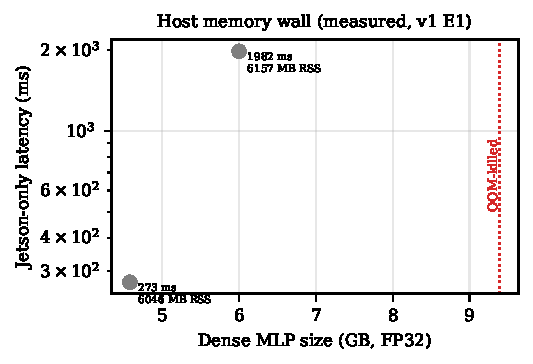
\includegraphics[width=0.95\columnwidth]{fig_capacity}
\caption{Jetson-only latency versus dense-model size (measured\M). Latency rises non-linearly at 6~GB and the process is killed at 9.39~GB.}
\label{fig:capacity}\end{figure}

\subsection{Two ways to use attached memory}
Given a memory node on a link of bandwidth $B$ and per-message latency $r$, a layer with $W$ weight bytes and $F$ floating-point operations can execute in one of three placements:
\begin{itemize}
\item \textbf{host}: weights resident in SoC memory, compute on the GPU; cost $F/G_{\text{gpu}}$; consumes $W$ of host memory.
\item \textbf{pool}: weights resident on the node; the host faults them in through \cxlwin{} and computes locally; cost $W/B + n_{\text{msg}} r + F/G_{\text{gpu}}$ with $n_{\text{msg}}$ the number of fault batches; consumes no persistent host memory.
\item \textbf{NMC}: weights resident on (or streamed to) the node; the node's engine computes; cost $S(W) + r + F/G_{\text{nmc}}$ where $S$ is the streaming cost, zero if the weights are already resident.
\end{itemize}
Pool moves memory to compute; NMC moves compute to memory. For resident weights the two are equal when
\begin{equation}
B^{*} \;=\; \frac{W}{\;F/G_{\text{nmc}} + r - F/G_{\text{gpu}} - n_{\text{msg}} r\;},
\label{eq:crossover}
\end{equation}
a per-layer crossover bandwidth. Above $B^{*}$ the link is fast enough that hauling weights to the faster GPU wins; below it, the slow engine next to the memory wins because it avoids the haul. \S\ref{sec:placement} uses (\ref{eq:crossover}) inside an exact placer; \S\ref{sec:results} checks it against executed latencies.

\subsection{CXL.mem as an analogy, software DSM as an ancestor}
CXL.mem gives a host cache-line-granular, hardware-coherent loads and stores to device memory; a Type~2 device additionally holds a \emph{bias} per page---host bias, where the host's caches are authoritative, or device bias, where the device may operate on the memory without snooping the host. \cxlwin{} reproduces the second idea faithfully and the first only at page granularity, in software, without hardware coherence. The mechanism---protect the pages, service faults by fetching over the network, track ownership in a per-page state machine---is that of Ivy~\cite{ivy}, Munin~\cite{munin} and TreadMarks~\cite{treadmarks}. We claim no novelty in the mechanism. What is new is using it as the \emph{memory-to-compute} arm of a controlled comparison against near-memory compute on the same device, over the same link, with the same program.

% ============================================================================
\section{Design}
\label{sec:design}

\begin{figure}[t]\centering
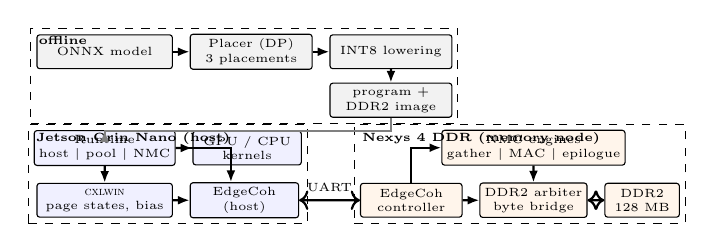
\begin{tikzpicture}[font=\tiny, node distance=2.5mm, scale=0.86, transform shape,
  box/.style={draw, rounded corners=1pt, minimum height=5mm, inner sep=2pt, align=center},
  host/.style={box, fill=blue!6}, dev/.style={box, fill=orange!8}, off/.style={box, fill=gray!10},
  arr/.style={-{Latex[length=1.5mm]}, thick}]
  % offline
  \node[off, minimum width=20mm] (onnx) {ONNX model};
  \node[off, right=of onnx, minimum width=18mm] (placer) {Placer (DP)\\3 placements};
  \node[off, right=of placer, minimum width=18mm] (lower) {INT8 lowering};
  \node[off, below=2mm of lower, minimum width=18mm] (prog) {program +\\DDR2 image};
  \draw[arr] (onnx)--(placer); \draw[arr] (placer)--(lower); \draw[arr] (lower)--(prog);
  \node[draw, dashed, fit=(onnx)(placer)(lower)(prog), inner sep=2pt, label={[anchor=north west]north west:\textbf{offline}}] {};
  % host
  \node[host, below=9mm of onnx, minimum width=20mm] (run) {Runtime\\host $|$ pool $|$ NMC};
  \node[host, below=of run, minimum width=20mm] (win) {\cxlwin{}\\page states, bias};
  \node[host, right=of win, minimum width=16mm] (ec) {EdgeCoh\\(host)};
  \node[host, right=of run, minimum width=16mm] (gpu) {GPU / CPU\\kernels};
  \draw[arr] (run)--(gpu); \draw[arr] (run)--(win); \draw[arr] (win)--(ec); \draw[arr] (run.east) -| ($(ec.north)+(-2mm,0)$);
  \node[draw, dashed, fit=(run)(win)(ec)(gpu), inner sep=2pt, label={[anchor=north west]north west:\textbf{Jetson Orin Nano (host)}}] {};
  % device
  \node[dev, right=9mm of ec, minimum width=15mm] (ctrl) {EdgeCoh\\controller};
  \node[dev, right=of ctrl, minimum width=15mm] (arb) {DDR2 arbiter\\byte bridge};
  \node[dev, above=of arb, minimum width=15mm] (nmc) {NMC engines\\gather $|$ MAC $|$ epilogue};
  \node[dev, right=of arb, minimum width=11mm] (ddr) {DDR2\\128 MB};
  \draw[arr, <->] (ec)--node[above, font=\tiny]{UART} (ctrl);
  \draw[arr] (ctrl)--(arb); \draw[arr] (ctrl)|-(nmc); \draw[arr] (nmc)--(arb); \draw[arr, <->] (arb)--(ddr);
  \node[draw, dashed, fit=(ctrl)(arb)(nmc)(ddr), inner sep=2pt, label={[anchor=north west]north west:\textbf{Nexys 4 DDR (memory node)}}] {};
  \draw[arr, gray] (prog.south) -- ++(0,-2mm) -| (run.north);
\end{tikzpicture}
\caption{SplitInfer. Offline: the placer chooses host/pool/NMC per layer and the lowering emits one INT8 program and DDR2 image. Online: the runtime executes the program in a mode; pool mode dereferences pointers into the \cxlwin{} window, whose page faults become EdgeCoh reads; NMC mode dispatches to the engines and reads back results.}
\label{fig:arch}\end{figure}

\subsection{\cxlwin{}: a load/store window with ownership}
\label{sec:cxlwin}
\cxlwin{} reserves a host virtual range the size of the device region with no access permission. A dereference faults; a handler that uses only async-signal-safe calls hands the address to a service thread, which performs the transfer, changes the page protection, and releases the faulting thread to re-execute the instruction. A store to a readable page faults a second time and upgrades the page to writable and dirty. Table~\ref{tab:states} lists the six page states and Fig.~\ref{fig:states} the transitions.

\begin{table}[t]\caption{\cxlwin{} page states}\label{tab:states}\centering\footnotesize
\begin{tabular}{@{}llp{4.3cm}@{}}\toprule
State & Protection & Meaning \\ \midrule
\textsc{invalid} & none & no valid host copy; device holds the data \\
\textsc{fetching} & none & \emph{transient}: a read is outstanding \\
\textsc{shared} & read & host holds a clean copy; device copy valid \\
\textsc{modified} & read/write & host copy dirty; device copy stale \\
\textsc{flushing} & read & \emph{transient}: a write-back is outstanding \\
\textsc{device} & none & device bias: an engine owns the page \\ \bottomrule
\end{tabular}\end{table}

\begin{figure}[t]\centering
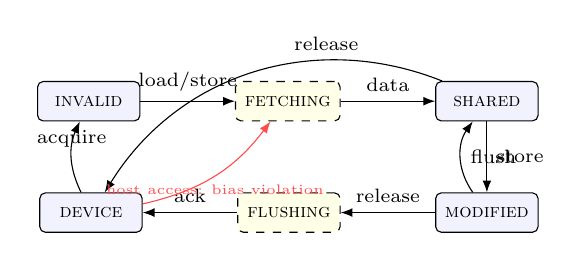
\begin{tikzpicture}[font=\scriptsize, >={Latex[length=1.5mm]}, node distance=9mm and 12mm,
  st/.style={draw, rounded corners=2pt, minimum width=13mm, minimum height=5mm, fill=blue!5},
  tr/.style={st, dashed, fill=yellow!10}]
  \node[st] (inv) {\textsc{invalid}};
  \node[tr, right=of inv] (fet) {\textsc{fetching}};
  \node[st, right=of fet] (sh) {\textsc{shared}};
  \node[st, below=of sh] (mod) {\textsc{modified}};
  \node[tr, left=of mod] (fl) {\textsc{flushing}};
  \node[st, left=of fl] (dev) {\textsc{device}};
  \draw[->] (inv)--node[above]{load/store} (fet);
  \draw[->] (fet)--node[above]{data} (sh);
  \draw[->] (sh)--node[right]{store} (mod);
  \draw[->] (mod)--node[above]{release} (fl);
  \draw[->] (fl)--node[above]{ack} (dev);
  \draw[->] (dev) to[bend left=25] node[above]{acquire} (inv);
  \draw[->] (sh) to[bend right=40] node[above, pos=0.3]{release} (dev);
  \draw[->] (mod) to[bend left=35] node[right]{flush} (sh);
  \draw[->, red!70] (dev) to[bend right=20] node[below, font=\tiny]{host access: bias violation} (fet);
\end{tikzpicture}
\caption{Page-state transitions. Dashed states are transient and exist only while a transfer is outstanding. A host access to a \textsc{device}-bias page is a coherence violation; by default it is counted and serviced, in strict mode it aborts.}
\label{fig:states}\end{figure}

\textbf{Ownership.} \texttt{release(range)} writes back \textsc{modified} pages and moves the range to \textsc{device}; the runtime calls it before dispatching an engine on that memory. \texttt{acquire(range)} moves \textsc{device} pages to \textsc{invalid}; the next host access re-fetches whatever the engine wrote. This is the CXL Type~2 bias flip, at page granularity and directed by software. The transient states matter for correctness: a second fault on a page whose read is outstanding must wait for that read, not issue another, and a \texttt{release} racing a fault must not write back a half-filled page. Both are guaranteed by holding the window's lock across the transient state.

\textbf{Prefetch.} A miss fetches $P$ contiguous pages in one message. $P{=}1$ is demand paging; larger $P$ amortises the per-message latency $r$ but fetches pages that may never be touched. \S\ref{sec:results} shows that this trade-off has a sign that depends on the layer.

\textbf{What \cxlwin{} is not.} It is not cache-line coherent, it does not snoop, and it does not make the device's memory appear in the host's physical address map. Its guarantee is weaker and explicit: between \texttt{release} and \texttt{acquire} the device's view is authoritative; outside that interval the host's view is. That is enough for layer-sequential inference and is stated as such.

\subsection{EdgeCoh: the message protocol}
EdgeCoh carries \cxlwin{}'s faults and the runtime's dispatches. Every message has an 8-byte header (type, flags, tensor id, payload length). \textsc{data\_write} and \textsc{data\_read} move bytes to and from DDR2 byte addresses; \textsc{nmc\_exec} carries an opcode and six 32-bit parameters; \textsc{sync\_barrier}, \textsc{transfer\_ownership} and \textsc{prefetch} are one-round-trip control messages; the device answers everything with \textsc{ack} or \textsc{data\_response}. The protocol is deliberately dumb: the intelligence is in \cxlwin{}'s state machine and the placer, not in the wire format.

\subsection{Near-memory engines}
Three engines operate on DDR2-resident INT8 tensors in the memory controller's clock domain (81.25~MHz):
\emph{gather} copies rows of an embedding table selected by INT32 indices;
\emph{INT8 FC} computes $y = W x$ for a row-major $W$ of $M{\times}K$ INT8 weights into INT32 accumulators with an 8$\times$8 array---eight independent lanes, each an 8-wide dot product, so that one 16-byte activation read is reused across eight weight rows;
\emph{epilogue} computes $\mathrm{sat}_8(\mathrm{relu}((y+b)\cdot m \gg s))$ with an INT32 bias $b$, a 16-bit multiplier $m$ and a shift $s$. The epilogue is the standard fixed-point requantisation, chosen precisely because a host can reproduce it bit for bit. Alignment rules (16-byte addresses, $K$ padded to 16, $M$ to 16) are imposed by the lowering, not the user.

\subsection{INT8 lowering and the program}
The lowering takes an ONNX graph and a placement and produces a \emph{program}---an ordered list of layer records with DDR2 addresses, dimensions and requantisation parameters---a DDR2 \emph{image} of INT8 tables and weights and INT32 biases, and a set of \emph{test vectors} with expected integer outputs. Activation scales are calibrated per tensor on random inputs through onnxruntime; \textsc{MatMul}$\rightarrow$\textsc{Add}$\rightarrow$\textsc{Relu} chains fuse into one FC record; \textsc{Concat} is made free by pinning each producer's output inside the concatenation buffer. The same program executes in every mode, and every mode is checked against the same expected integers.

\subsection{Placement}
\label{sec:placement}
The placer is an exact dynamic program over (layer, placement, host-memory-used, device-memory-used), with memory tracked in adaptive buckets and an argmin table for backtracking. The cost of a layer in a placement is the sum in \S\ref{sec:background}; a change of compute location between consecutive layers adds an activation crossing. Two constraints bound it: host-resident weights must fit a host budget, and device-resident weights must fit device memory---either individually (streamed) or cumulatively (resident). The DP is verified against exhaustive enumeration on small instances. Its parameters are meant to be measured: the artifact ships a calibration script that fits $B$ and $r$ from the link, and the engine rate comes from cycle-accurate simulation of the MAC data path (0.684~MAC/cycle, \CDlrmFpgaGops~GOPS at 81.25~MHz).

The placer operates on the ONNX graph, before fusion. Its per-layer decisions and crossover bandwidths are reported (\S\ref{sec:results}); the runtime in this paper executes whole programs in one mode at a time, and executing a mixed placement layer by layer is future work.

% ============================================================================
\section{Implementation and Verification}
\label{sec:impl}

\textbf{FPGA.} The design runs in two clock domains bridged by handshake CDCs and gray-code FIFOs: a 100~MHz domain for the UART and the EdgeCoh controller, and the MIG's 81.25~MHz domain for a DDR2 arbiter and the engines. The arbiter owns the MIG user interface, converts byte addresses to the controller's 16-bit-word address space, holds commands until the controller accepts them, tags the single outstanding read with its owner, queues two writes per engine port, and bridges the controller's byte stream to 128-bit bursts with a byte-masked write assembler and a one-word read cache that preserves read-after-write ordering.

\textbf{Host.} \cxlwin{} and EdgeCoh are C; the lowering and placer are Python; the runtime and kernels are C++. The runtime's three executors share one set of integer kernels: the host executor runs them on host-resident weights, the pool executor runs the same kernels on pointers into the \cxlwin{} window, and the NMC executor sends dispatches.

\textbf{Virtual FPGA.} The EdgeCoh transport is a small vtable, and a second implementation of it is an in-process device model: 128~MB of DDR2 as a byte array and the three engines with the RTL's integer semantics, plus an emulated link (bandwidth, per-message latency) and emulated engine time (cycle counts from simulation). Everything above the transport---runtime, \cxlwin{}, lowering---is byte-for-byte identical between the emulator and the board. Numbers from the emulator are labelled \E{} and are never presented as measurements.

\textbf{Verification.} Four testbenches under Icarus Verilog drive the RTL with random operands against reference computations---a DMA byte round trip through unaligned addresses with guard bytes, a 24$\times$48 INT8 matrix-vector product, a 32-row gather, and a 44-element epilogue with a partial tail---and the virtual FPGA passes the same vectors through the protocol API. The lowering's reference executor, the host executor, the pool executor and the NMC executor are then required to produce identical INT32 outputs on every test vector; a mismatch fails the run. Table~\ref{tab:e2} reports that check for every cell.

\textbf{What golden vectors found.} The v1 design had passed functional simulation and a hardware loopback test that compared only message headers. Golden vectors found that its engines passed byte addresses into the memory controller's word-unit address space, that its byte-stream writes zeroed fifteen neighbouring bytes and its byte reads always returned lane~0 of a burst, that its gather always selected the first index of each 16-byte word, and that its MAC array broadcast one dot product to all eight accumulators. None of these could have been caught by a test that checks acknowledgements. The board then found two more that simulation had passed: the UART transmitter's ready flag is registered and stays high for one cycle after accepting a byte, so the response-header state emitted every second byte; and the memory controller's read-data bus is valid only in the cycle its valid flag is high, whereas the behavioural model held the last value---the gather engine copied a cycle late and every embedding row came back wrong while the pool path, which reads through the DMA bridge, was bit-exact. Both were reproduced in simulation only after the model was made as strict as the silicon. We record this as the methodological lesson of the project: for a memory node, the test that matters is the one that reads back what it wrote, and the model must be at least as unforgiving as the hardware about \emph{when} data is valid.

% ============================================================================
\section{Methodology}
\label{sec:method}

\textbf{Platform.} Jetson Orin Nano Super (JetPack~6, R36.5, TensorRT~10.7, CUDA~12.6); Digilent Nexys~4 DDR (XC7A100T, 128~MB DDR2) over an FT2232HQ UART at 115{,}200 baud, 8N1 (11{,}520~B/s ceiling). All host-side numbers are taken on the Jetson.

\textbf{Workloads.} A synthetic DLRM~\cite{dlrm}: 26 embedding tables of $1000{\times}64$, a 128-feature dense input, and a $1792{\to}1024{\to}256{\to}1$ top MLP (36 ONNX nodes, \CDlrmWeightsMiB~MiB FP32, \PDlrmImageMiB~MiB INT8). Dense MLPs of $5000{\times}5000$ layers for the capacity experiments. Weights are seeded random ($\mathcal{N}(0,1/\sqrt{\text{fan-in}})$); an earlier version of this work used all-zero weights, which invalidates any correctness check and makes INT8 quantisation degenerate.

\textbf{Baselines.} B1: onnxruntime FP32 on the CPU. B2: onnxruntime dynamic INT8 on the CPU. B3: TensorRT FP16 on the GPU. B4: TensorRT INT8 on the GPU (implicit quantisation; a timing baseline, not an accuracy one). B3 and B4 are new; the earlier version had only CPU baselines because the installed onnxruntime has no CUDA provider.

\textbf{Measurement.} Every cell is 30 measured iterations after 5 warm-ups, wrapped in a tegrastats window stretched to at least 3~s so that power rests on dozens of samples; a cell that fails or times out is recorded as such. We report medians with p99, coefficient of variation, and maximum---never a median alone. Energy per inference is mean power times mean latency. Correctness is a bit-exact comparison of INT32 outputs against the lowering's expected values, plus the normalised error of the dequantised output against FP32 onnxruntime.

\textbf{Claims.} Each number carries a provenance mark: \M{} measured on hardware, \E{} produced by the virtual FPGA with an emulated link, \Cm{} from the cost model. At the time of writing the FPGA data path has been re-synthesised but the board measurements of the v2 design are pending; every SplitInfer latency in this version is therefore \E, and the UART point of Fig.~\ref{fig:crossover} is the one the board will anchor.

% ============================================================================
\section{Results}
\label{sec:results}

\subsection{E2: every path on one workload}
Table~\ref{tab:e2} and Fig.~\ref{fig:e2} put every execution path on the DLRM at batch~1. Three things are worth reading off. First, the model fits in host memory, so it \emph{should not} be disaggregated, and the placer says so: with a normal host budget it places all 36 nodes on the host (\Cm). The SplitInfer rows exist to price the mechanism, not to recommend it here. Second, the INT8 host path is \MEmulSIhostMedian~ms---slower than the FP16 GPU's \MEmulBthreetrtfponesixgpuMedian~ms because it is a scalar CPU kernel; the interesting comparison is between the three SplitInfer modes, which share that kernel. Third, at UART speed NMC costs \EEmulSInmcMedian~ms and demand-paged pool \EEmulSIpoolMedian~ms: a 560$\times$ gap between the two ways of using the same memory node over the same link, with identical outputs (\EEmulSInmcBitExact{} and \EEmulSIpoolBitExact{} bit-exact).

\begin{table*}[t]\caption{E2: DLRM, batch 1, 30 iterations. Latency per inference; link traffic per inference; bit-exact agreement with expected INT32 output. Provenance: \M{} measured, \E{} emulated link at UART parameters (11{,}520~B/s, 5~ms RTT).}\label{tab:e2}\centering\footnotesize
\begin{tabular}{@{}llrrrrrrrr@{}}\toprule
Path & Prov. & Median (ms) & p99 (ms) & CV (\%) & Power (mW) & Energy (mJ) & Link out / in (B) & Msgs & Bit-exact \\ \midrule
B1 onnxruntime FP32, CPU & \M & \MEmulBoneortfpthreetwocpuMedian & \MEmulBoneortfpthreetwocpuPninenine & -- & \MEmulBoneortfpthreetwocpuPower & \MEmulBoneortfpthreetwocpuEnergy & -- & -- & -- \\
B2 onnxruntime INT8, CPU & \M & \MEmulBtwoortinteightcpuMedian & \MEmulBtwoortinteightcpuPninenine & -- & \MEmulBtwoortinteightcpuPower & \MEmulBtwoortinteightcpuEnergy & -- & -- & -- \\
B3 TensorRT FP16, GPU & \M & \MEmulBthreetrtfponesixgpuMedian & \MEmulBthreetrtfponesixgpuPninenine & \MEmulBthreetrtfponesixgpuCV & \MEmulBthreetrtfponesixgpuPower & \MEmulBthreetrtfponesixgpuEnergy & -- & -- & -- \\
B4 TensorRT INT8, GPU & \M & \MEmulBfourtrtinteightgpuMedian & \MEmulBfourtrtinteightgpuPninenine & \MEmulBfourtrtinteightgpuCV & \MEmulBfourtrtinteightgpuPower & \MEmulBfourtrtinteightgpuEnergy & -- & -- & -- \\ \midrule
SI host (INT8, host-resident) & \M & \MEmulSIhostMedian & \MEmulSIhostPninenine & \MEmulSIhostCV & \MEmulSIhostPower & \MEmulSIhostEnergy & 0 / 0 & 0 & \MEmulSIhostBitExact \\
SI NMC (compute $\to$ memory) & \E & \EEmulSInmcMedian & \EEmulSInmcPninenine & \EEmulSInmcCV & \EEmulSInmcPower & \EEmulSInmcEnergy & \EEmulSInmcLinkOut{} / \EEmulSInmcLinkIn & \EEmulSInmcMsgs & \EEmulSInmcBitExact \\
SI pool, 64-page prefetch & \E & \EEmulSIpoolMedian & \EEmulSIpoolPninenine & \EEmulSIpoolCV & \EEmulSIpoolPower & \EEmulSIpoolEnergy & 0 / \EEmulSIpoolLinkIn & \EEmulSIpoolFaults & \EEmulSIpoolBitExact \\
SI pool, warm (host-cached) & \E & \EEmulSIpoolwarmMedian & \EEmulSIpoolwarmPninenine & \EEmulSIpoolwarmCV & \EEmulSIpoolwarmPower & \EEmulSIpoolwarmEnergy & 0 / \EEmulSIpoolwarmLinkIn & \EEmulSIpoolwarmFaults & \EEmulSIpoolwarmBitExact \\ \bottomrule
\end{tabular}\end{table*}

\begin{figure}[t]\centering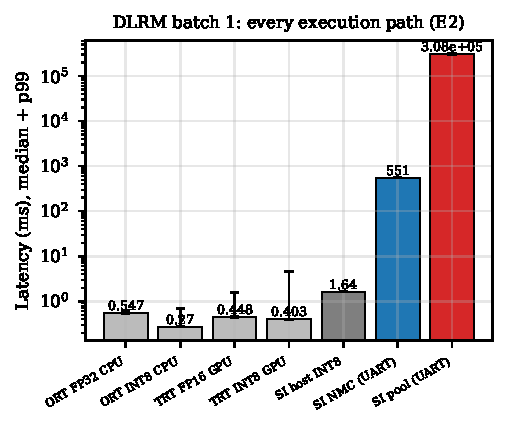
\includegraphics[width=0.95\columnwidth]{fig_e2}
\caption{E2 latencies (log scale; bar = median, whisker to p99).}
\label{fig:e2}\end{figure}

\textbf{Weight staging is a first-class cost.} Before any inference the \PDlrmImageMiB~MiB image must reach DDR2; at UART speed that takes \EEmulSInmcPrepare~s. The previous version of this work excluded it from every reported latency. It is reported here as preparation time and, for the streaming case (\S\ref{sec:capacity}), inside the per-inference latency where it belongs.

\subsection{E6: the crossover}
Fig.~\ref{fig:crossover} runs the same program in NMC and pool modes with the emulated link set to six classes from UART to PCIe~4$\times$4 (Table~\ref{tab:e6}). NMC flattens at ${\sim}\Esixpciefourxfournmc$~ms, the engines' compute time; the link only ever costs it 59 small messages. Pool falls with bandwidth until it meets the host-resident floor. The two cross between USB~2.0 (\Esixusbtwobulknmc{} vs \Esixusbtwobulkpoolpfsixfour~ms, NMC wins) and USB~3 (\Esixusbthreenmc{} vs \Esixusbthreepoolpfsixfour~ms, pool wins): on this workload, moving compute to memory pays below roughly $10^8$~bytes/s and stops paying above it. Equation~(\ref{eq:crossover}) gives per-layer crossovers of 89~MB/s for the gathers and 196~MB/s for the 7~MB MatMul with the calibrated parameters---the right decade, bracketing the executed crossover.

\begin{figure}[t]\centering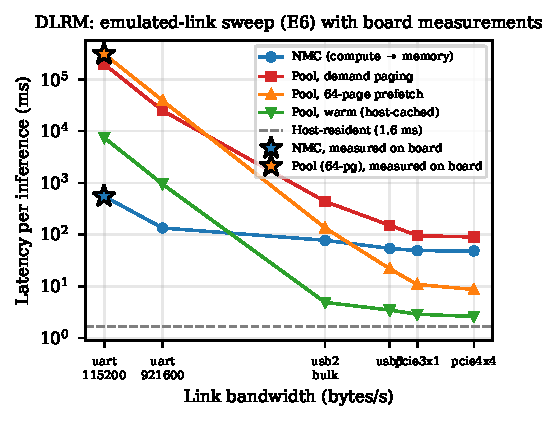
\includegraphics[width=0.95\columnwidth]{fig_crossover}
\caption{E6 (\E): latency per inference versus link bandwidth for NMC and three pool configurations. The crossover between NMC and prefetching pool lies between USB~2.0 and USB~3.}
\label{fig:crossover}\end{figure}

\begin{table}[t]\caption{E6 (\E): median latency per inference (ms) across link classes.}\label{tab:e6}\centering\footnotesize
\resizebox{\columnwidth}{!}{\begin{tabular}{@{}lrrrrr@{}}\toprule
Link & NMC & Pool $P{=}1$ & Pool $P{=}64$ & Pool $P{=}512$ & Pool warm \\ \midrule
UART 115.2k & \Esixuartoneonefivetwozerozeronmc & \Esixuartoneonefivetwozerozeropoolpfone & \Esixuartoneonefivetwozerozeropoolpfsixfour & \Esixuartoneonefivetwozerozeropoolpffiveonetwo & \Esixuartoneonefivetwozerozeropoolwarm \\
UART 921.6k & \Esixuartninetwoonesixzerozeronmc & \Esixuartninetwoonesixzerozeropoolpfone & \Esixuartninetwoonesixzerozeropoolpfsixfour & \Esixuartninetwoonesixzerozeropoolpffiveonetwo & \Esixuartninetwoonesixzerozeropoolwarm \\
USB 2.0 bulk & \Esixusbtwobulknmc & \Esixusbtwobulkpoolpfone & \Esixusbtwobulkpoolpfsixfour & \Esixusbtwobulkpoolpffiveonetwo & \Esixusbtwobulkpoolwarm \\
USB 3 & \Esixusbthreenmc & \Esixusbthreepoolpfone & \Esixusbthreepoolpfsixfour & \Esixusbthreepoolpffiveonetwo & \Esixusbthreepoolwarm \\
PCIe 3 $\times$1 & \Esixpciethreexonenmc & \Esixpciethreexonepoolpfone & \Esixpciethreexonepoolpfsixfour & \Esixpciethreexonepoolpffiveonetwo & \Esixpciethreexonepoolwarm \\
PCIe 4 $\times$4 & \Esixpciefourxfournmc & \Esixpciefourxfourpoolpfone & \Esixpciefourxfourpoolpfsixfour & \Esixpciefourxfourpoolpffiveonetwo & \Esixpciefourxfourpoolwarm \\ \bottomrule
\end{tabular}}\end{table}

\textbf{Prefetch has a sign.} At UART speed a 64-page prefetch is \emph{slower} than demand paging (Table~\ref{tab:e6}, first row) even though it makes 14 round trips instead of \EsixuartoneonefivetwozerozeropoolpfoneFaults. Each gather touches one 256-byte row of a 256~KB table; a 256~KB prefetch fetches the whole table. On a bandwidth-bound link the wasted bytes dominate; on a latency-bound link the saved round trips dominate, and the order reverses from USB~2.0 upward. The right prefetch depth is a property of the layer's access pattern, which the placer knows and a page-fault handler does not.

\textbf{Warm pool is not host-resident.} With host copies retained across inferences, pool converges toward the host floor but never reaches it, because successive inputs select different embedding rows and each new row faults. For sparse layers the pool's steady-state cost is the input's locality, not the model's size.

\subsection{E7: capacity, executed}
\label{sec:capacity}
An eight-layer $5000{\times}5000$ MLP has \PMlpEightTotalWeightMiB~MiB of INT8 weights---larger than the FPGA's 128~MB. Lowered with streaming, its FC layers rotate through two \PMlpEightSlotMiB~MiB slots and the runtime downloads each layer's weights immediately before dispatching it; the peak DDR2 footprint is \PMlpEightLayoutMiB~MiB. The program runs end to end, bit-exact against the reference (\EsevennmcnolinkBitExact), with normalised error \EsevennmcnolinkNormErr{} against FP32. Its price is stated in Table~\ref{tab:e7}: at USB~2.0 rates, \EsevennmcusbtwoStream~ms of every \EsevennmcusbtwoMedian~ms inference is weight streaming; at USB~3, \EsevennmcusbthreeStream~ms of \EsevennmcusbthreeMedian~ms. The capacity multiplier a streaming design earns is total weight divided by $2\times$ the largest layer, and it is bought with $W_{\text{total}}/B$ per inference. Over a UART link that is hours per inference; over PCIe it is tens of milliseconds. Whether it is worth buying is, again, a property of the link.

\begin{table}[t]\caption{E7 (\E): 8-layer MLP, \PMlpEightTotalWeightMiB~MiB INT8 $>$ 128~MB DDR2, streamed through 2$\times$\PMlpEightSlotMiB~MiB slots.}\label{tab:e7}\centering\footnotesize
\begin{tabular}{@{}lrrl@{}}\toprule
Mode / link & Latency (ms) & of which streaming & Bit-exact \\ \midrule
Host-resident & \EsevenhostMedian & -- & \EsevenhostBitExact \\
NMC, no link delay & \EsevennmcnolinkMedian & \EsevennmcnolinkStream & \EsevennmcnolinkBitExact \\
NMC, USB 2.0 bulk & \EsevennmcusbtwoMedian & \EsevennmcusbtwoStream & \EsevennmcusbtwoBitExact \\
NMC, USB 3 & \EsevennmcusbthreeMedian & \EsevennmcusbthreeStream & \EsevennmcusbthreeBitExact \\ \bottomrule
\end{tabular}\end{table}

\subsection{Cost model against execution}
For the DLRM with host budget zero and resident weights, the placer chooses \CDlrmNumFpga{} NMC layers, \CDlrmNumPool{} pool layer (a 4-byte bias, where one page fault beats one dispatch) and \CDlrmNumGpu{} host layers with no weights, and estimates \CDlrmLatency~ms (\Cm); the executed NMC program runs in \EEmulSInmcMedian~ms (\E). The model's dispatch and compute terms (\CDlrmBddispatch{} and \CDlrmBdfpgacompute~ms) match execution to within 30\%; its overestimate is the activation crossing it charges at the \textsc{Concat} (\CDlrmBdactivationxfer~ms), which the lowering removes by pinning producers into the concatenation buffer. A placer on the lowered program rather than the ONNX graph would close that gap; we leave it as stated.

\subsection{Accuracy}
Per-tensor symmetric INT8 with the fused fixed-point epilogue reproduces FP32 outputs to a normalised error of \PDlrmNormErr{} on the DLRM and \PMlpEightNormErr{} on the eight-layer MLP. The point of the scheme is not its accuracy but its determinism: host, pool and NMC agree to the bit.

% ============================================================================
\section{Discussion}
\label{sec:discussion}

\textbf{When does compute-to-memory win?} Below the crossover---here $10^7$--$10^8$~bytes/s---and only if the weights are already resident on the node; a design that must stream weights every inference pays $W/B$ either way and NMC's advantage collapses to the difference between engine and GPU compute time, which the GPU wins. Above the crossover, pool wins, and a node with no engines at all---a plain memory expander with a good link---is the right design. The value of NMC at the edge is therefore bounded by the slowness of edge links, which is a statement about today's edge I/O, not about NMC.

\textbf{What the UART substrate is for.} It is the worst case, chosen so that every protocol cost is visible at millisecond scale. It is not proposed as a deployment. The sweep in Fig.~\ref{fig:crossover} is the deployment guidance: it says which class of link makes which design correct.

\textbf{Limitations.} (1)~SplitInfer latencies in this version are emulated; the board run of the v2 data path is the outstanding measurement, and the emulator's engine timing is calibrated from simulation, not silicon. (2)~The runtime executes one mode for a whole program; mixed per-layer placements are modelled, not executed. (3)~Batch size is one; the MAC engine reuses activations across eight rows but not weights across samples. (4)~INT8 per-tensor quantisation is the only precision. (5)~Pool-mode compute runs on the CPU; a GPU pool path would add a host-to-device copy of the faulted pages, which the E2 GPU baselines show to be ${\sim}0.1$~ms at this size.

% ============================================================================
\section{Related Work}
\textbf{Software DSM} supplied the mechanism: Ivy~\cite{ivy} (sequentially consistent page-based DSM), Munin~\cite{munin} (multiple consistency protocols), TreadMarks~\cite{treadmarks} (lazy release consistency). \cxlwin{} is a single-writer, release-consistent window with explicit ownership transfer---closest to Munin's write-shared protocol with the release directed by a scheduler rather than by locks.
\textbf{CXL} memory systems---Pond~\cite{pond_cxl}, TPP~\cite{tpp_cxl}, DirectCXL~\cite{cxl_type2}---assume a coherent link of ${\sim}10^{10}$~bytes/s; this paper is about what happens three to six decades below that.
\textbf{Weight streaming} for models larger than accelerator memory---FlexGen~\cite{flexgen}, ZeRO-Inference~\cite{zero_inference}, PowerInfer~\cite{powerinfer}---moves weights to the GPU from host memory or SSD and overlaps it with compute; those systems are pool-mode designs at $10^9$--$10^{10}$~bytes/s and our results agree that pool is right there.
\textbf{Near-memory and processing-in-memory}---HBM-PIM~\cite{hbm_pim}, UPMEM~\cite{upmem}, and the survey of Ghose \emph{et al.}~\cite{nmc_survey}---place compute beside memory to avoid a bandwidth wall inside a package; we place it beside memory to avoid a bandwidth wall on a cable, and find the same rule with a different constant.
\textbf{FPGA inference}---Vitis~AI~\cite{vitis_ai}, FINN~\cite{finn}, hls4ml~\cite{hls4ml}---treats the FPGA as an accelerator; our engines are deliberately small, because the question is where compute should sit, not how fast an FPGA can be.
\textbf{Edge partitioning}---Neurosurgeon~\cite{neurosurgeon}, DADS~\cite{dads}, DeepThings~\cite{deepthings}---partitions compute across devices by latency; our placer partitions \emph{residency} under two memory constraints with three placements, and its distinguishing output is a crossover bandwidth per layer.

% ============================================================================
\section{Conclusion}
For a model that does not fit an edge SoC, the choice between moving memory to compute and compute to memory is decided by the link. We built both over one commodity substrate---a page-granular load/store window with explicit ownership, and near-memory INT8 engines---made them execute the same program to the same integers, and measured the crossover by running it: below about $10^8$~bytes/s the engines next to the memory win, above it the link is fast enough to haul weights to the GPU, and a capacity-unlocking streaming design pays $W/B$ per inference in either case. The artifact reproduces every number here from its data files, and the board run of the verified data path is the next measurement.

\section*{Acknowledgments}
The author used Claude Code (Anthropic) as a software-engineering assistant during the v2 rebuild. All design decisions, experiments and interpretations are the author's.

\begin{thebibliography}{20}
\bibitem{ivy} K.~Li and P.~Hudak, ``Memory coherence in shared virtual memory systems,'' \emph{ACM Trans. Comput. Syst.}, vol.~7, no.~4, pp.~321--359, 1989.
\bibitem{munin} J.~B. Carter, J.~K. Bennett, and W.~Zwaenepoel, ``Implementation and performance of Munin,'' in \emph{Proc. SOSP}, 1991, pp.~152--164.
\bibitem{treadmarks} P.~Keleher, A.~L. Cox, S.~Dwarkadas, and W.~Zwaenepoel, ``TreadMarks: Distributed shared memory on standard workstations and operating systems,'' in \emph{Proc. USENIX Winter}, 1994, pp.~115--131.
\bibitem{cxl_type2} D.~Gouk \emph{et al.}, ``Direct access, high-performance memory disaggregation with DirectCXL,'' in \emph{Proc. USENIX ATC}, 2022, pp.~287--304.
\bibitem{pond_cxl} H.~Li \emph{et al.}, ``Pond: CXL-based memory pooling systems for cloud platforms,'' in \emph{Proc. ASPLOS}, 2023, pp.~574--587.
\bibitem{tpp_cxl} H.~Al~Maruf \emph{et al.}, ``TPP: Transparent page placement for CXL-enabled tiered memory,'' in \emph{Proc. ASPLOS}, 2023, pp.~742--755.
\bibitem{flexgen} Y.~Sheng \emph{et al.}, ``FlexGen: High-throughput generative inference of large language models with a single GPU,'' in \emph{Proc. ICML}, 2023.
\bibitem{zero_inference} R.~Y. Aminabadi \emph{et al.}, ``DeepSpeed-Inference: Enabling efficient inference of transformer models at unprecedented scale,'' in \emph{Proc. SC}, 2022.
\bibitem{powerinfer} Y.~Song \emph{et al.}, ``PowerInfer: Fast large language model serving with a consumer-grade GPU,'' in \emph{Proc. SOSP}, 2024.
\bibitem{hbm_pim} S.~Lee \emph{et al.}, ``Hardware architecture and software stack for PIM based on commercial DRAM technology,'' in \emph{Proc. ISCA}, 2021, pp.~43--56.
\bibitem{upmem} J.~Devaux, ``The true processing in memory accelerator,'' in \emph{Proc. Hot Chips}, 2019.
\bibitem{nmc_survey} S.~Ghose \emph{et al.}, ``Processing-in-memory: A workload-driven perspective,'' \emph{IBM J. Res. Dev.}, vol.~63, no.~6, 2019.
\bibitem{vitis_ai} Xilinx, ``Vitis AI,'' 2023.
\bibitem{finn} Y.~Umuroglu \emph{et al.}, ``FINN: A framework for fast, scalable binarized neural network inference,'' in \emph{Proc. FPGA}, 2017, pp.~65--74.
\bibitem{hls4ml} J.~Duarte \emph{et al.}, ``Fast inference of deep neural networks in FPGAs for particle physics,'' \emph{JINST}, vol.~13, no.~7, 2018.
\bibitem{neurosurgeon} Y.~Kang \emph{et al.}, ``Neurosurgeon: Collaborative intelligence between the cloud and mobile edge,'' in \emph{Proc. ASPLOS}, 2017, pp.~615--629.
\bibitem{dads} L.~Zeng \emph{et al.}, ``DADS: Device-aware DNN splitting for edge inference,'' in \emph{Proc. SEC}, 2020.
\bibitem{deepthings} Z.~Zhao \emph{et al.}, ``DeepThings: Distributed adaptive deep learning inference on resource-constrained IoT edge clusters,'' \emph{IEEE TCAD}, vol.~37, no.~11, pp.~2348--2359, 2018.
\bibitem{dlrm} M.~Naumov \emph{et al.}, ``Deep learning recommendation model for personalization and recommendation systems,'' arXiv:1906.00091, 2019.
\end{thebibliography}

\begin{IEEEbiographynophoto}{Hemraj Lamkuche}
is a researcher in heterogeneous computing and FPGA-based edge ML inference systems.
\end{IEEEbiographynophoto}
\end{document}
